\chapter{Introduction}
\label{ch:into} % This how you label a chapter and the key (e.g., ch:into) will be used to refer this chapter ``Introduction'' later in the report. 
% the key ``ch:into'' can be used with command \ref{ch:intor} to refere this Chapter.

With the rise of digital transactions, the chances of online fraud have also increased 
significantly. Credit cards have become an integral part of financial transactions which facilitates online commerce more easily and it is also convenient for customers. However, with an increase in the use of such online transactions, there is an increase in the risk of fraud which leads to huge losses for both customers and financial institutions. Credit card fraud happens when an unidentified user makes the transaction using someone else’s card information.
Detecting such fraud manually is a very challenging task due to such a high number of transactions every moment. To deal with this cybercrime, an efficient fraud detection system \citep{Dornadula-2019} should be established which uses various machine learning algorithms and models to accurately detect the fraud. In this research, a credit card fraud detection dataset  is taken from an online source Kaggle \citep{Kaggle}  where the data is cleaned and processed to extract relevant information which can be used as training data for the machine learning models to accurately detect the fraud. Some machine learning algorithms \citep{Shah-2023} that are used are logistic regression,decision tree classification, and random forest classification which can detect fraud based on the data of past transactions and can detect fraud in real-time which is a big advantage of using machine learning algorithms. After that, these models are further tuned for provided dataset  using techniques like hyperparameter tuning \citep{Dalal-2022} , which greatly enhances the model's performance. The training data used in these models are based on various factors like location, date and time of the transaction, past transactions, etc. The performance of these combined models is then evaluated using various evaluation metrics. Deployment of such fraud detection systems ensures safer transactions by improving online security.




%%%%%%%%%%%%%%%%%%%%%%%%%%%%%%%%%%%%%%%%%%%%%%%%%%%%%%%%%%%%%%%%%%%%%%%%%%%%%%%%%%%
\section{Background}
\label{sec:into_back}

With the rise of digital transactions, the risk of credit card fraud has escalated. Current 
fraud detection systems are struggling to keep pace with evolving tactics, prompting 
the need for more efficient solutions. This study utilizes machine learning algorithms such as 
Logistic Regression and Decision Trees to craft a responsive credit card fraud 
detection system. Prioritizing real-time adaptability, the project seeks to enhance the 
security of financial transactions, contributing to the ongoing battle against credit card 
fraud.

%%%%%%%%%%%%%%%%%%%%%%%%%%%%%%%%%%%%%%%%%%%%%%%%%%%%%%%%%%%%%%%%%%%%%%%%%%%%%%%%%%%
\section{Problem statement}
\label{sec:intro_prob_art}
Credit card fraud is a major financial problem because it can be tough to identify and results in significant difficulties for individuals, businesses, and financial institutions. Fraudsters attempt to avoid the system and make unauthorised purchases with another person's credit card illegally using their card information which is confidential and can be easily misused. Not only does this harm the individual whose card is taken, but it also causes significant financial losses to banks and retailers. Thus, a sophisticated system that can identify suspicious credit card transactions is needed to ensure that people's money is safe and that everyone may use credit cards without fear of criminals seeking to take advantage of them.

%%%%%%%%%%%%%%%%%%%%%%%%%%%%%%%%%%%%%%%%%%%%%%%%%%%%%%%%%%%%%%%%%%%%%%%%%%%%%%%%%%%
\section{Aims and objectives}
\label{sec:intro_aims_obj}

The main purpose of this research is to assess the performance of the user's fraud detection model utilizing various supervised machine algorithms and deep learning and artificial neural models to increase the accuracy of the model and gain a higher detection accuracy by comparing alternative approaches. A credit card fraud detection system's goal is to provide a clever and effective system that can easily identify and avoid illegal or unauthorized credit card transactions. Therefore, creating a system that can identify anomalous behaviors or fraud transactions and promptly notify individuals and financial institutions of such activities is the primary goal.



%%%%%%%%%%%%%%%%%%%%%%%%%%%%%%%%%%%%%%%%%%%%%%%%%%%%%%%%%%%%%%%%%%%%%%%%%%%%%%%%%%%
\section{Solution approach}
\label{sec:intro_sol} % label of Org section
Credit Card Fraud Detection is a vital component of guaranteeing financial security for customers and companies alike. It becomes evident that traditional machine learning techniques have not been able to provide effective solutions by analyzing the difficulties related to credit card fraud, such as the availability of public data, class imbalance in data, the changing nature of frauds, and the high number of false alarms. It is possible to create fraud detection algorithms that are more precise and efficient, though, given the recent developments in deep learning. These technologies will save financial organizations billions of dollars that are lost annually to fraud, as well as provide employment security and secure bank and credit card earnings. To improve the productivity and usefulness of its findings, the research incorporates several models. A hybrid strategy is chosen among the models examined, which include Regression-based classifiers, Decision Tree classifiers, and Boosting based models. This hybrid method optimizes using a grid-based searching algorithm and combines a tree-based model with a linear-based model. The models are optimized to maximize performance on the given dataset using methods like hyperparameter tuning. However, determining the best set of hyperparameters may be difficult and time-consuming, particularly when dealing with a wide variety of hyperparameters and intricate models like LightGBM and XGBoost. The training of the tress by gradient boost technique is optimised by the use of XG Boost which is an Extreme Gradient Boosting algorithm. It is monitored and incredibly adaptable and effective. Large data sets may be utilized for regression and classification and it has an ease of managing the missing values very well by the use of regularization techniques L1 and L2. Improvements have been demonstrated in these areas: accuracy, sensitivity, and precision by evaluating the model on certain performance metrics like recall or precision scores, F1 measures, false negatives and false positives, etc. 

Thus, by enhancing safety measures, this technology gives the banking industry a better way to identify and stop scams during online transactions.

 

\subsection{Flow Chart of Data}
\label{sec:intro_some_sub1}


Below, we see how we process the data for our Model Evaluation.

\begin{figure}[ht]
    \centering
    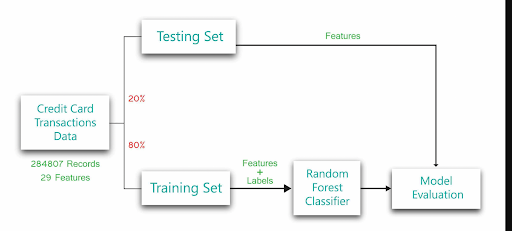
\includegraphics[scale=0.3]{figures/FlowOfData.png}
    \caption{Figure of the Data}
    \label{fig:Plot of the Data}
\end{figure}

\subsection{A subsection 2}
\label{sec:intro_some_sub2}
Depending on your project's needs, add more section(s) and subsection(s).

\subsubsection{A subsection 1 of a subsection}
\label{sec:intro_some_subsub1}
The command \textbackslash subsubsection\{\} creates a paragraph heading in \LaTeX.

\subsubsection{A subsection 2 of a subsection}
\label{sec:intro_some_subsub2}
Write your text here...

%%%%%%%%%%%%%%%%%%%%%%%%%%%%%%%%%%%%%%%%%%%%%%%%%%%%%%%%%%%%%%%%%%%%%%%%%%%%%%%%%%%
\section{Summary of contributions and achievements} %  use this section 
\label{sec:intro_sum_results} % label of summary of results
Describe clearly what you have done/created/achieved and what the major results and their implications are. 


%%%%%%%%%%%%%%%%%%%%%%%%%%%%%%%%%%%%%%%%%%%%%%%%%%%%%%%%%%%%%%%%%%%%%%%%%%%%%%%%%%%

